\begin{graphicspathcontext}{{./chapters/simulation/imgs/},{./chapters/simulation/imgs/auto/},\old}

\begin{frame}{SARL and CArtAgO}
	\begin{columns}[T]
		\begin{column}{.5\linewidth}
			\begin{block}{SARL + A\&A}
				SARL integrates with CArtAgO through dedicated \emph{capacities} and \emph{skills} that allow agents to:
				\begin{itemize}
				\item Create/lookup artifacts
				\item Execute operations on artifacts
				\item Observe artifact properties via events
				\end{itemize}
			\end{block}
		\end{column}
		\begin{column}{.5\linewidth}
			\begin{block}{Mapping to A\&A}
				\begin{itemize}
				\item An \emph{agent} = a SARL \code{agent}
				\item \emph{Capacities/Skills} implement how the agent \emph{interacts with artifacts}
				\item \emph{Events} carry percepts from artifact observable properties and signals
				\item \emph{Environment} = CArtAgO workspaces
				\end{itemize}
			\end{block}
		\end{column}
	\end{columns}
	\begin{center}
		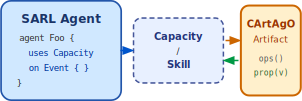
\includegraphics[width=.5\linewidth]{artefact_sarl_aa}
	\end{center}
\end{frame}

\begin{frame}[t,fragile]{{SARL:} Defining a Capacity for Artifact Interaction}
	\begin{sarllisting}[basicstyle=\scriptsize]
/** Capacity to interact with the Counter artifact. */
capacity Counter {

	/** Create a link to a counter artifact. */
	def makeCounter(name : String) : ArtifactId

	/** Listening artefact events. */
	def focusCounter(id : ArtifactId) : ArtifactId

	/** Increment the counter. */
	def increment(artifactId : ArtifactId)

	/** Reset the counter to zero. */
	def resetCounter(artifactId : ArtifactId)

	/** Read the current count value. */
	def getCount(artifactId : ArtifactId) : int
}
	\end{sarllisting}
	\vspace{-1cm}
	\begin{itemize}
	\item Capacities \Emph{decouple} the agent from the artifact implementation
	\item Skill provides the \Emph{concrete bridge} to CArtAgO operations
	\end{itemize}
\end{frame}

\begin{frame}[t,fragile]{{SARL:} Defining a Capacity for Artifact Workspace}
	\begin{sarllisting}[basicstyle=\scriptsize]
/** Capacity to set-up the A&A workspace. */
capacity CArtAgO {

	/** Reply the workspace identifier from a name. */
	def getWorkspaceId(name : String) : WorkspaceId

	/** Create a link to an artefact. */
	def makeArtifact(name : String, type : String) : ArtifactId

	/** Execute operation on artefact. */
	def execLinkedOp(id : ArtifactId, name : String, param : Object*)	

	/** Listening artefact events. */
	def focus(id : ArtifactId) : ArtifactId

}
	\end{sarllisting}
	\vspace{-1cm}
	\begin{itemize}
	\item Capacity provides the bridge to the base CArtAgO API
	\end{itemize}
\end{frame}

\begin{frame}[t,fragile]{{SARL:} Implementing the Skill (CArtAgO bridge)}
	\begin{sarllisting}[basicstyle=\scriptsize]
skill CounterArtefact implements Counter {
	uses CArtAgO
	def makeCounter(name : String) : ArtifactId {
		makeArtifact(name, "demo.counter.CounterArtifact")
	}
	def focusCounter(artifactId : ArtifactId) : ArtifactId {
		focus(artifactId)
	}
	def increment(artifactId : ArtifactId) : ArtifactId {
		// Delegate to the CArtAgO artifact operation
		execLinkedOp(artifactId, "inc")
	}
	def resetCounter(artifactId : ArtifactId) : ArtifactId {
		owner.execLinkedOp(artifactId, "reset")
	}
	def getCount(artifactId : ArtifactId) : int {
		val v = newArrayOfSize(1)
		execLinkedOp(artifactId, "getValue", v)
		return v.get(0) as Integer
	}
}
	\end{sarllisting}
\end{frame}

\begin{frame}[t,fragile]{{SARL:} Writing the Agent}
	\vspace{-.25cm}
	\begin{sarllisting}[basicstyle=\scriptsize]
agent CounterAgent {
	uses Counter, CArtAgO, Logging

	on Initialize {
		// 1. Equip the agent with the corresponding skill
		setSkill(new CounterArtefact)

		// 2. Join the CArtAgO workspace
		val wid = "default".workspaceId

		// 3. Create (or lookup) the Counter artifact
		val aid = "myCounter".createCounter

		// 4. Use artifact operations via the capacity
		aid.increment.increment.increment
		info("Counter value = " + aid.count) // prints: 3

		aid.resetCounter
		info("After reset = " + aid.count) // prints: 0
	}
}
	\end{sarllisting}
\end{frame}

\begin{frame}[t,fragile]{{SARL} Observing an Artifact (Percepts as Events)}
	\begin{sarllisting}[basicstyle=\tiny]
/** Event generated by A&A layer when an observable property changes. */
event CountChanged {
	val artifactId : ArtifactId
	val newValue : int
}

agent ObservingAgent {
	uses Counter, CArtAgO, Logging

	on Initialize {
		// 1. Equip the agent with the corresponding skill
		setSkill(new CounterArtefact)

		// 2. Join the CArtAgO workspace
		val wid = "default".workspaceId

		// 3. Create (or lookup) the Counter artifact
		val aid = "myCounter".createCounter

		// Focus = subscribe to observable property changes
		aid.focusCounter
	}

	/** Reacts to observable property change: count(N). */
	on CountChanged {
		info("Perceived count change -> " + occurrence.newValue)
	}

}
	\end{sarllisting}
\end{frame}

\end{graphicspathcontext}
